\subsection{UC 4: Logout}
		
		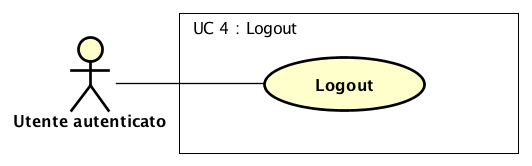
\includegraphics[scale=0.8]{../../Casi D'uso/UC4.png}
\begin{itemize}
		\item \textbf{Attori coinvolti:} Utente autenticato. \\
		\item \textbf{Scopo e descrizione:} L'utente autenticato pu\'o eseguire il logout dall’applicazione. \\
		\item \textbf{Precondizione:} L'applicazione offre all'utente la possibilit\'a di logout. \\
		\item \textbf{Postcondizione:}L'applicazione ha eseguito l'operazione di logout richiesta dall’utente. \\
\end{itemize}